\documentclass{beamer}
\usepackage[utf8]{inputenc}
\usepackage{graphicx}

\title{Topluluk Tespiti: Klasik Algoritmalar ve Çizge Sinir Ağları Karşılaştırması}
\author{Emre YILDIZ}
\institute{Ege Üniversitesi \\ Bilgisayar Mühendisliği Bölümü}
\date{\today}

\usetheme{Madrid}
\usecolortheme{beaver}

\begin{document}

\begin{frame}
    \titlepage
\end{frame}

\begin{frame}{Proje Hakkında}
    \begin{itemize}
        \item \textbf{Ders:} Cebirsel Çizge Algoritmaları (Yüksek Lisans)
        \item \textbf{Amaç:} Çizge Teorisi'nin teorik temellerini modern Makine Öğrenmesi uygulamaları ile birleştiren kapsamlı bir topluluk tespiti (community detection) çalışmasıdır.
        \item \textbf{Yöntemler:} Neo4j ve PyTorch kullanarak klasik algoritmaları (Louvain, LPA) Graph Neural Networks (GCN, GraphSAGE, GAT) ile karşılaştırmak.
        \item \textbf{Veriseti:} Cora Citation Network.
    \end{itemize}
\end{frame}

\begin{frame}{Kullanılan Kütüphane ve Araçlar}
    \begin{itemize}
        \item \textbf{Neo4j (GDS):} Yüksek performanslı çizge veritabanı. Louvain ve Label Propagation gibi klasik topluluk tespit algoritmalarını çalıştırmak için kullanıldı.
        \item \textbf{PyTorch (PyG):} Derin öğrenme ve özellikle Çizge Sinir Ağları (GNN) modelleri oluşturmak ve eğitmek için kullanılan esnek bir kütüphane.
        \item \textbf{NetworkX:} Çizge oluşturma, manipülasyonu ve temel çizge metriklerinin hesaplanması için kullanıldı.
        \item \textbf{Scikit-learn:} GNN modellerinin performansını değerlendirmek için Adjusted Rand Index (ARI) ve Normalized Mutual Information (NMI) gibi metriklerin hesaplanmasında kullanıldı.
        \item \textbf{Seaborn \& Matplotlib:} Veri ve sonuçların görselleştirilmesi, karşılaştırma grafikleri oluşturulması için kullanıldı.
    \end{itemize}
\end{frame}

\begin{frame}{Neo4j ve Graph Data Science (GDS) Rolü}
    \framesubtitle{Projedeki İşlevi ve İş Akışı}
    \begin{itemize}
        \item \textbf{Veri Depolama ve Modelleme:} Cora veriseti, Neo4j'de çizge yapısına en uygun şekilde depolanmıştır:
        \begin{itemize}
            \item Düğümler: \texttt{:Paper} etiketi ile makaleler.
            \item İlişkiler: \texttt{[:CITES]} ilişkisi ile makaleler arası alıntılar.
        \end{itemize}
        \item \textbf{In-Memory Çizge Projeksiyonu:} Analizden önce, GDS kütüphanesi ile \texttt{'cora-graph'} adında bir "in-memory" yansıtma oluşturulur. Bu, algoritmaların disk I/O olmadan çok yüksek hızda çalışmasını sağlar.
        \item \textbf{Klasik Algoritmaların Çalıştırılması:}
        \begin{itemize}
            \item \texttt{gds.louvain.write(...)} ve \texttt{gds.labelPropagation.write(...)} fonksiyonları ile topluluk tespiti algoritmaları çalıştırılmıştır.
            \item \texttt{writeProperty} parametresi sayesinde, her bir algoritmanın bulduğu topluluk kimliği (\texttt{louvainCommunityId}, \texttt{lpaCommunityId}) doğrudan ilgili düğümlerin bir özelliği olarak veritabanına geri yazılmıştır.
        \end{itemize}
        \item \textbf{Entegrasyon Noktası:} Neo4j, hem klasik algoritmaların analiz merkezi hem de PyTorch ile eğitilen GNN modelleri için bir veri kaynağı görevi görmüştür.
    \end{itemize}
\end{frame}

\begin{frame}{Louvain Algoritması}
    \begin{columns}[T]
        \begin{column}{.5\textwidth}
            \textbf{Çalışma Prensibi:}
            \begin{itemize}
                \item Hiyerarşik bir kümeleme algoritmasıdır ve amacı ağdaki modülerlik skorunu maksimize etmektir.
                \item \textbf{1. Aşama (Modülerlik Optimizasyonu):} Her düğüm, komşu düğümlerin bulunduğu toplulukları tek tek dener. Düğüm, modülerlikte en büyük artışı sağlayan topluluğa taşınır. Bu işlem, hiçbir düğüm hareketi modülerliği artırmayana kadar tekrarlanır.
                \item \textbf{2. Aşama (Topluluk Birleştirme):} İlk aşamada bulunan topluluklar, tek birer "süper düğüm" olarak kabul edilir ve bu süper düğümler arasında yeni bir ağ oluşturulur.
                \item Bu iki aşama, ağ yapısında bir değişiklik olmayana kadar tekrarlanır.
            \end{itemize}
        \end{column}
        \begin{column}{.5\textwidth}
            \begin{figure}
                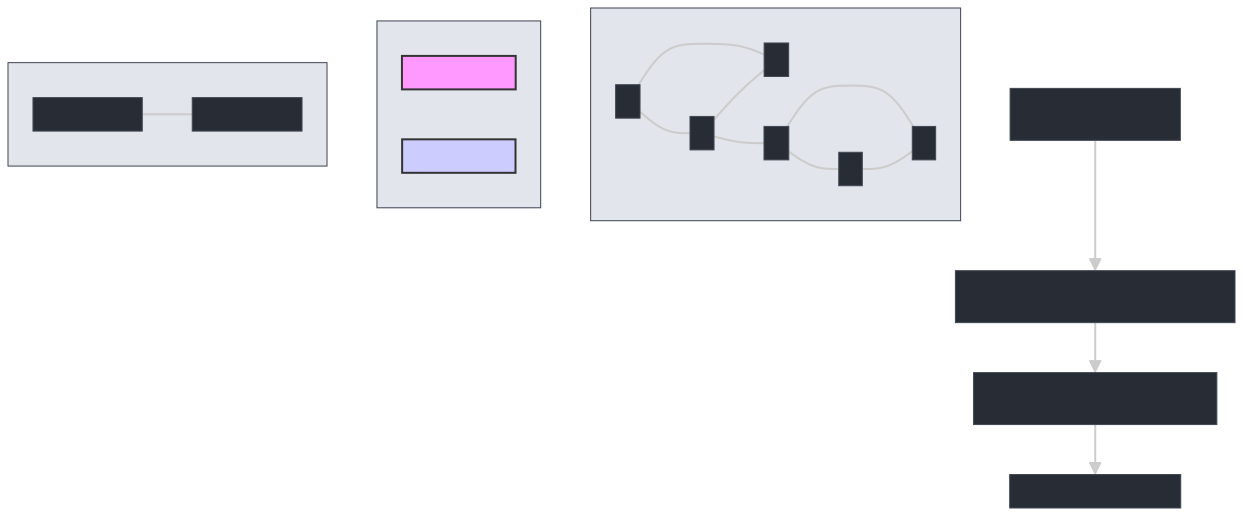
\includegraphics[width=\textwidth]{images/louvain.jpg}
                \caption{Louvain algoritmasının iki aşamalı yapısı.}
            \end{figure}
        \end{column}
    \end{columns}
\end{frame}

\begin{frame}{Label Propagation (LPA)}
    \begin{columns}[T]
        \begin{column}{.5\textwidth}
            \textbf{Çalışma Prensibi:}
            \begin{itemize}
                \item Yarı denetimli bir algoritmadır ve düğümlerin etiketlerini komşularına yayarak toplulukları bulur.
                \item \textbf{Başlangıç:} Her düğüme benzersiz bir etiket atanır.
                \item \textbf{İterasyon:} Her adımda, her düğüm komşularının etiketlerine bakar ve komşuları arasında en sık görülen (majoritary) etiketi kendi etiketi olarak günceller.
                \item \textbf{Duruş Kriteri:} Bu işlem, hiçbir düğümün etiketini değiştirmediği bir denge durumuna ulaşılana kadar tekrarlanır.
                \item Sonuç olarak, aynı etikete sahip düğümler bir topluluk oluşturur.
            \end{itemize}
        \end{column}
        \begin{column}{.5\textwidth}
            \begin{figure}
                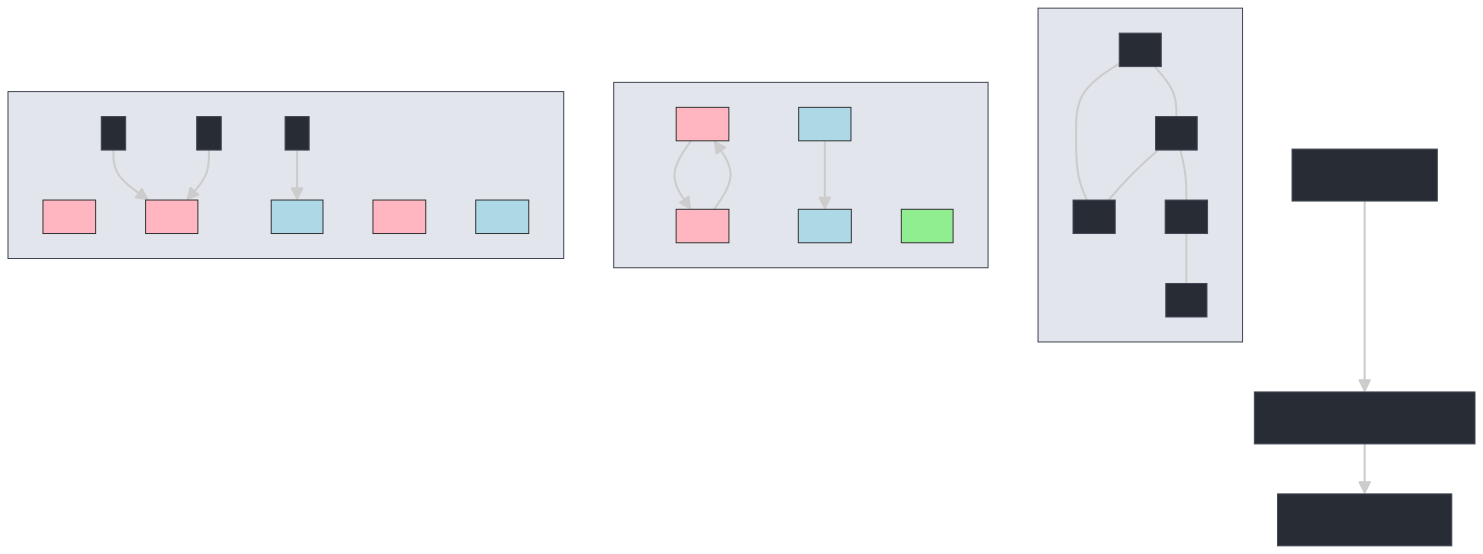
\includegraphics[width=\textwidth]{images/lpa_diagram.jpg}
                \caption{Etiketlerin komşular arasında yayılması.}
            \end{figure}
        \end{column}
    \end{columns}
\end{frame}

\begin{frame}{Graph Convolutional Network (GCN)}
    \begin{columns}[T]
        \begin{column}{.5\textwidth}
            \textbf{Çalışma Prensibi:}
            \begin{itemize}
                \item Çizge evrişim (convolution) operatörünü kullanarak düğüm temsillerini (embeddings) öğrenir.
                \item Her katmanda, bir düğüm kendi komşu düğümlerinin özellik vektörlerini toplar (aggregation) ve ortalamasını alır.
                \item Bu toplanan bilgi, düğümün kendi özellik vektörü ile birleştirilir.
                \item Sonuç, bir aktivasyon fonksiyonundan (örneğin ReLU) geçirilerek düğümün yeni katmandaki temsili oluşturulur.
                \item Bu süreç, katman sayısı kadar tekrarlanarak daha geniş komşuluklardan bilgi toplanması sağlanır.
            \end{itemize}
        \end{column}
        \begin{column}{.5\textwidth}
            \begin{figure}
                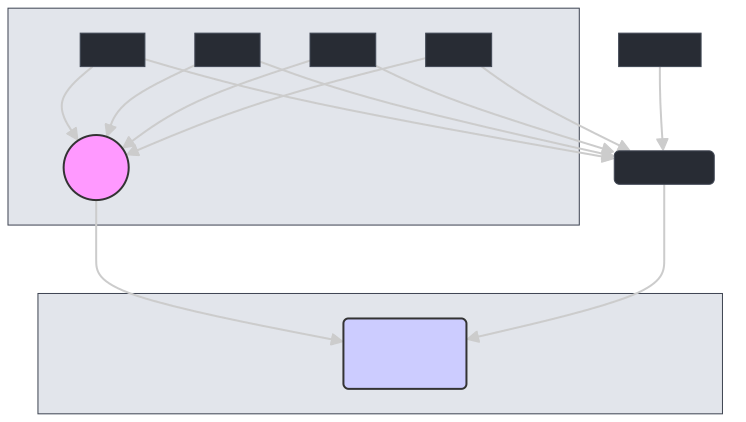
\includegraphics[width=\textwidth]{images/gcn_diagram.jpg}
                \caption{Komşuluk bilgilerinin toplanması ve güncellenmesi.}
            \end{figure}
        \end{column}
    \end{columns}
\end{frame}

\begin{frame}{GraphSAGE}
    \begin{columns}[T]
        \begin{column}{.5\textwidth}
            \textbf{Çalışma Prensibi:}
            \begin{itemize}
                \item "Sample and Aggregate" (Örnekle ve Birleştir) fikrine dayanır ve büyük çizgeler için tasarlanmıştır.
                \item \textbf{Örnekleme:} Her düğüm için tüm komşuları kullanmak yerine, sabit sayıda komşu rastgele örneklenir. Bu, hesaplama maliyetini düşürür.
                \item \textbf{Birleştirme (Aggregation):} Örneklenen komşuların özellik vektörleri bir birleştirme fonksiyonu (örneğin, Mean, Max-Pooling veya LSTM) kullanılarak tek bir vektörde birleştirilir.
                \item \textbf{Güncelleme:} Bu birleştirilmiş vektör, hedef düğümün kendi mevcut vektörü ile birleştirilerek düğümün yeni temsili oluşturulur.
            \end{itemize}
        \end{column}
        \begin{column}{.5\textwidth}
            \begin{figure}
                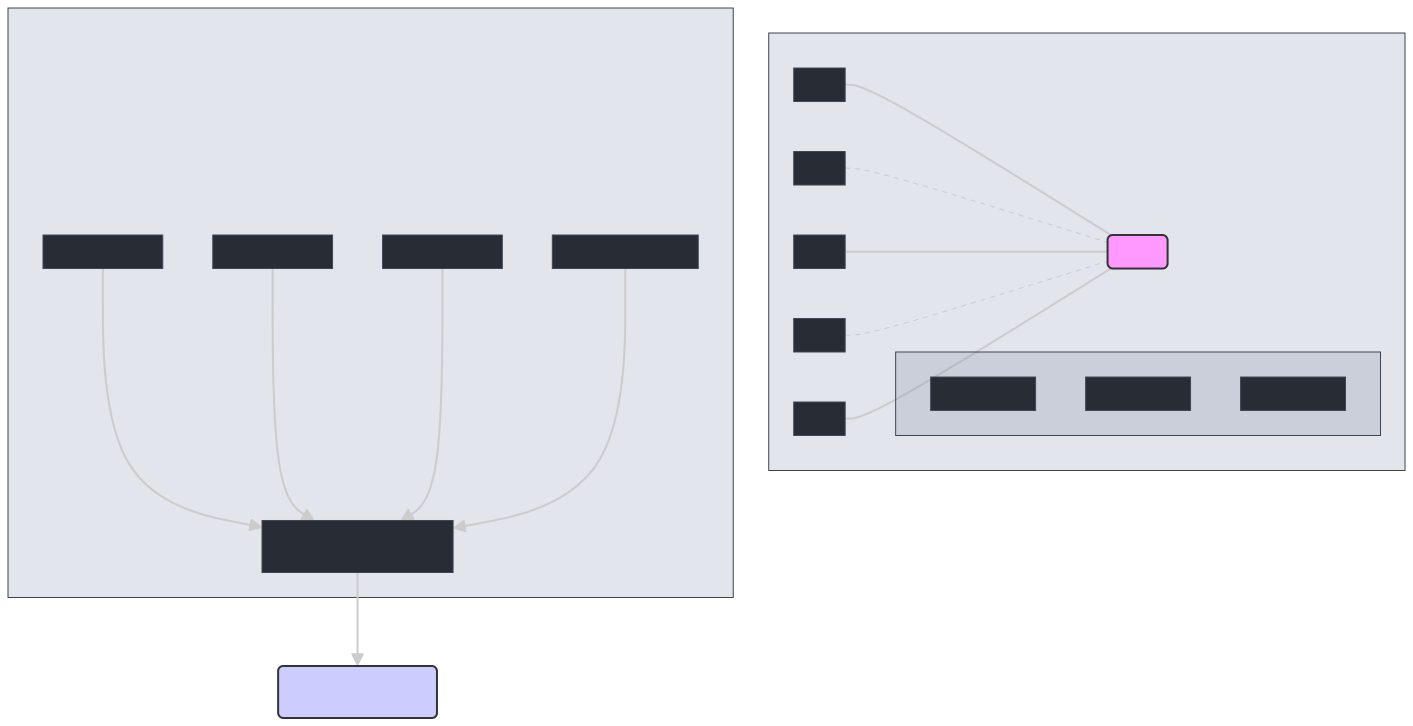
\includegraphics[width=\textwidth]{images/graphsage_diagram.jpg}
                \caption{Komşulardan örnekleme ve bilgiyi birleştirme.}
            </end{figure}
        </end{column}
    \end{columns}
\end{frame}

\begin{frame}{Graph Attention Network (GAT)}
    \begin{columns}[T]
        \begin{column}{.5\textwidth}
            \textbf{Çalışma Prensibi:}
            \begin{itemize}
                \item Komşu düğümlerin bilgilerini birleştirirken dikkat (attention) mekanizmasını kullanır.
                \item GCN ve GraphSAGE'in aksine, her komşuya eşit önem vermek yerine, her komşuya bir "dikkat skoru" (attention score) atar.
                \item Bu skorlar, hedef düğüm için hangi komşuların daha önemli olduğunu belirtir ve ağırlıklı bir ortalama alınmasını sağlar.
                \item Bu sayede model, daha ilgili komşulara odaklanarak daha zengin ve anlamlı düğüm temsilleri öğrenebilir.
                \item Maskelenmiş dikkat (masked attention) sayesinde sadece komşuluk bilgisi kullanılır.
            \end{itemize}
        \end{column}
        \begin{column}{.5\textwidth}
            \begin{figure}
                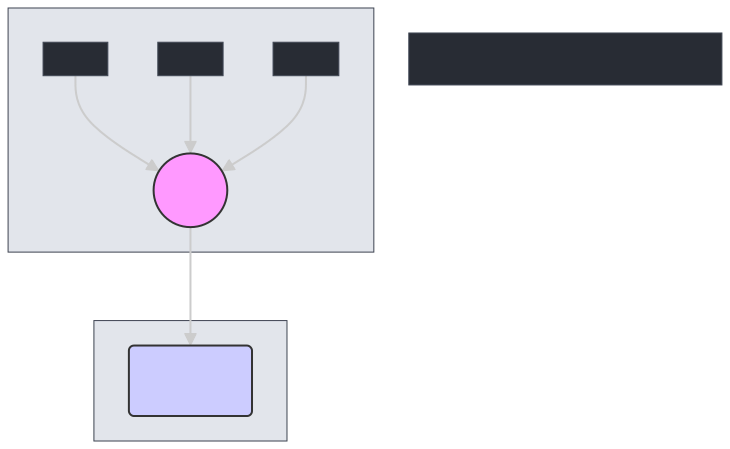
\includegraphics[width=\textwidth]{images/gat_diagram.jpg}
                \caption{Komşulara dikkat skorları ile ağırlıklandırma.}
            </end{figure}
        </column}
    \end{columns}
\end{frame}

\begin{frame}{Sonuçlar: Veriseti İstatistikleri}
    \begin{figure}
        \includegraphics[width=\textwidth]{../results/dataset_stats.png}
        \caption{Cora verisetinin temel istatistikleri ve derece dağılımı.}
    \end{figure}
\end{frame}

\begin{frame}{Sonuçlar: Topluluk Karşılaştırması}
    \begin{figure}
        \includegraphics[width=\textwidth]{../results/community_comparison.png}
        \caption{Farklı algoritmalar tarafından tespit edilen topluluk sayılarının karşılaştırması.}
    \end{figure}
\end{frame}

\begin{frame}{Sonuçlar: Değerlendirme Metrikleri}
    \begin{figure}
        \includegraphics[width=\textwidth]{../results/evaluation_metrics.png}
        \caption{Algoritmaların ARI, NMI ve Modülerlik metriklerine göre performans karşılaştırması.}
    \end{figure}
\end{frame}

\begin{frame}{Sonuçlar: t-SNE ile Düğüm Gösterimi (Figure 1)}
    \begin{figure}
        \includegraphics[width=\textwidth]{../results/Figure_1.png}
        \caption{GCN modeli tarafından öğrenilen düğüm gömülmelerinin (embeddings) t-SNE ile 2 boyuta indirgenmiş hali.}
    \end{figure}
\end{frame}

\begin{frame}{Sonuçlar: t-SNE ile Düğüm Gösterimi (Figure 2)}
    \begin{figure}
        \includegraphics[width=\textwidth]{../results/Figure_2.png}
        \caption{GraphSAGE modeli tarafından öğrenilen düğüm gömülmelerinin (embeddings) t-SNE ile 2 boyuta indirgenmiş hali.}
    \end{figure}
\end{frame}

\begin{frame}{Teşekkürler}
    \centering
    \Huge
    Teşekkürler
\end{frame}

\end{document}
